\documentclass{book}
\usepackage[utf8]{inputenc}
\usepackage[english,ngerman]{babel}
\usepackage{datetime}
\usepackage{graphicx}
\usepackage{xspace}
\usepackage{hyperref}
\usepackage{listings}

\newdateformat{germanDate}{\twodigit{\THEDAY}.\twodigit{\THEMONTH}.\THEYEAR}

% eigene Commands
\newcommand{\sketchup}{\texttt{SketchUp}\xspace}
\newcommand{\rubyXL}{\texttt{rubyXL}\xspace}
\newcommand{\inifile}{\texttt{inifile}\xspace}

%\setcounter{secnumdepth}{0}
\begin{document}
	
	\begin{titlepage}
	\centering
	
\includegraphics{pics/sketchup-icon}\par\vspace{1cm}
	%		{\scshape\LARGE Columbidae University \par}
	
	\vspace{1.5cm}
	{\huge\bfseries Robers' Excel Convert\par}
	\vspace{1cm}
	{\scshape\Large - Anleitung -\par}
	\vspace{2cm}
	{\Large\itshape Timo Bergerbusch\par}
	\vfill
	im Auftrag von:\par
	Max Robers
	
	\vfill
	
	{\large \germanDate\today\par}
\end{titlepage}
	
	\tableofcontents
	\chapter{Einleitung}
	
	\chapter{RobersExcelConvert}
	\chapter{Voraussetzungen}
		\section{\sketchup Version}
		\section{Ruby Version}
		\section{Ruby Console} \label{Ruby Console}
		\section{Bibliotheken installieren} \label{Installation}
			Im Laufe des Programms werden zwei Bibliotheken verwendet:\\
			\begin{itemize}
				\item[] rubyXL
				\item[] inifile
			\end{itemize}		
				
			\subsection{\rubyXL} \label{rubyXL}
				Das \rubyXL-Gem wird verwendet um die Excel-Datei, welche die Stückzahl und die Bauteile der Transportkisten erstellt, zu lesen. Dies ist notwendig um eine Automatisierung zu ermöglichen und eine manuelle Übertragung zu umgehen.\\
				Das Gem kann innerhalb von \sketchup installiert werden. Dazu wir die \hyperref[Ruby Console]{Ruby Console} benötigt. in welche der Befehl:
				\hspace*{2cm}\lstinputlisting[xleftmargin=0.2\textwidth,xrightmargin=0.2\textwidth]{listings/installGem-rubyXL.txt}
				In folge der Installation des \rubyXL-Gems werden weitere Gems transitiv installiert, welche für die Ausführung von \rubyXL gebraucht werden.\\
				Eine vollständiger transitiver Abhängigkeitsgraph ist in \ref{Abhaengigkeitsgraph} gegeben.
			\subsection{\inifile} \label{inifile}
				Das \inifile-Gem 
				\hspace*{2cm}\lstinputlisting[xleftmargin=0.2\textwidth,xrightmargin=0.2\textwidth]{listings/installGem-inifile.txt}
				
			\begin{figure}
				\centering
				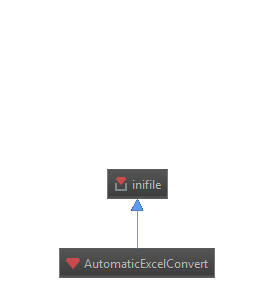
\includegraphics[scale=0.6]{pics/Gemdependency-full.png} %TODO: redraw
				\caption{Der Abhängigkeitsgraph der Gems}
				\label{Abhaengigkeitsgraph}
			\end{figure}
			
			
		\section{Gem einfügen}
			
		\section{Funktionstest}
	\chapter{Excel-Datei}
		\section{Aufbau}
		\section{Anpassungsmöglichkeiten}
	\chapter{Bauteil Identifizierung}
		\section{Translations}
			\subsection{Hinzufügen}
			\subsection{Aufbau}
			\subsection{Löschen}
	\chapter{Fehlerbehandlung}
		\section{Fehlercodes}
			\subsection*{Code: 0x00}
\end{document}